\documentclass{article}

\usepackage[francais]{babel}
\usepackage[T1]{fontenc}
\usepackage{geometry}
\geometry{hmargin=2.5cm}
\usepackage{amsmath}
\usepackage{graphicx}
\usepackage{subcaption}
\usepackage{float}
\PassOptionsToPackage{hyphens}{url}\usepackage{hyperref}
\usepackage{setspace}
\usepackage{siunitx}



\title{Capteurs 2019 -- 2020\bigbreak \bigbreak
    \large Dossier synthétique concernant des capteurs\\
    utilisant l’un des effets suivants :\bigbreak
    \normalsize effet thermoélectrique -- effet pyroélectrique -- effet piézoélectrique \\
    effet photoélectrique -- effet Hall -- effet photovoltaïque -- effet photoémissif\bigbreak}

\date{23 mars 2020}
\author{Laura Binacchi}

\begin{document}
    \pagenumbering{gobble}
    \maketitle
    \newpage
    \tableofcontents
    \newpage
    \pagenumbering{arabic}

    \newpage
    \section*{Introduction}
    \paragraph{}
    Ce travail traite des capteurs actifs au travers de septs effets physiques qu'ils mettent couramment en \oe uvre pour fonctionner : les effets thermoélectrique, pyroélectrique, piézoélectrique, photoélectrique, Hall, photovoltaïque et photoémissif.

    \paragraph{}
    Les capteurs actifs jouent le rôle de générateur dans les circuits électriques, contrairement aux capteurs passifs qui devaient être connectés à un générateur pour pouvoir fournir une information. Les capteurs actifs transforment l'énergie du mesurande en énergie électrique dont la variation nous fournit l'information sur le mesurande. Une exception est toutefois à faire pour l'effet Hall qui ne convertit pas l'énergie mais où un courant électrique est nécessaire pour produire une tension en fonction de la position d'un aimant.

    \paragraph{}
    Les grandeurs physiques mesurées par les effets étudiés dans ce travail sont la température (effet thermoélectrique), le flux de rayonnement optique (effets pyroélectrique, photovoltaïque, photoélectrique et photoémissif), la position (effet Hall) et la force, la pression ou l'accélération (effet piézoélectrique).

    \paragraph{}
    Pour chaque effet physique étudié, ce travail donnera d'abord une brève description de l'effet. Ensuite, deux capteurs industriels seront comparés et le fonctionnement de l'un des deux sera expliqué plus précisément sur base de schémas de documentation fournis par le fabricant.


    \newpage
    \section{Effet thermoélectrique}

    \subsection{Définition}
    \paragraph{}
    Il existe plusieurs effets thermoélectriques. Dans le domaine métrologique, ce lui qui nous intéresse est l'effet Seebeck qui concerne la transformation de chaleur en tension.

    \paragraph{}
    Dans un montage thermoélectrique de base, deux matériaux conducteurs de nature différente (a et b) sont reliées par deux jonctions (X et Y). Lorsque X et Y sont soumis à une différence de température $\Delta \theta$ une différence de potentiel $V_{AB}$ apparaît entre A et B. Cette différence de potentiel est liée à la différence de température par le coefficient Seebeck $S_{ab}$ dépendant de la nature des deux matériaux utilisés : $$V_{AB} = S_{ab} . \Delta \theta$$

    \begin{figure}[H]
        \centering
        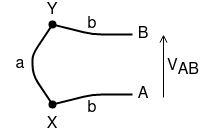
\includegraphics[width=0.2\linewidth]{./images/seedbeck.png}
    \end{figure}

    \paragraph{}
    L'effet Seebeck est principalement utilisé en thermométrie avec les thermocouples. Dans un thermocouple, la température d'une des deux jonctions est généralement connue et sert de référence pour déterminer la température de la seconde jonction. Les thermocouples sont classés en différents types en fonction du couple de matériau qui les compose : E (Chromel/Constantant), J (Fer/Constantan), T (Cuivre/Constantan), etc.

        \subsection{Thermocouples}
        \paragraph{}
        J'ai choisi deux thermocouples fabriqués par \href{https://new.abb.com/}{ABB}, qui en plus de fournir les datasheets des thermocouples, nous fournit \href{https://search-ext.abb.com/library/Download.aspx?DocumentID=03%2fTEMP-EN&LanguageCode=en&DocumentPartId=&Action=Launch}{un document} très utile pour l'utilisation des thermocouples en général. En effet, pour chaque type de thermocouple, ce sont des normes qui définissent la table de valeurs de la force électromotrice en fonction de la température et l'équation algébrique correspondant. En effet, les caractéristiques des thermocouples ne dépendent pas du fabricant mais sont principalement réglementées par des normes (e.g. les normes EN 60584 ou ANSI MC96-1 pour le type K).

        \subsubsection{Référence}
        \url{https://new.abb.com/products/measurement-products/temperature/high-temperature-thermometers/sensytemp-tsh200}

        \subsubsection{Comparaison de deux thermocouples}
        \begin{table}[H]
        \centering
        \begin{tabular}{l|c|c}
            \textbf{Modèle} & \textbf{TSH210 type K classe 1} & \textbf{TSH220  de type S classe 1}\\
            & 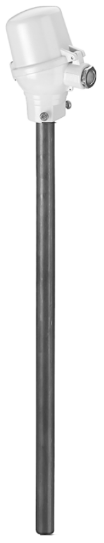
\includegraphics[width=0.05\linewidth]{./images/thermocouple-TSH210.png} & 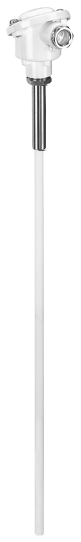
\includegraphics[width=0.04\linewidth]{./images/thermocouple-TSH220.png}\\
            \hline
            \textbf{Application}        & Fours de réchauffage et de durcissement, & Fabrication de ciment et de briques,   \\
                                        & fonderies, hauts fourneaux, incinération & industrie de la porcelaine et de la    \\
                                        & des déchets, désulfurisation des fumées  & céramique, incinération des déchets et \\
                                        &                                          & des déchets dangereux, industrie du    \\
                                        &                                          & verre, industrie de l'acier            \\
            \hline
            \textbf{Matériau de la}     & Métal                                     & Céramique\\
            \textbf{sonde (externe)}    & & \\
            \hline
            \textbf{Couple de}          & \multicolumn{1}{l|}{Métaux usuels :}               & \multicolumn{1}{l}{Métaux nobles :}\\
            \textbf{matériaux}          & \multicolumn{1}{l|}{ - Chromel (nickel/chrome)}    & \multicolumn{1}{l}{ - Platine-rhodium (10\%)}\\
                                        & \multicolumn{1}{l|}{ - Alumel (nickel/aluminimum)} & \multicolumn{1}{l}{ - Platine}\\
            \hline
            \textbf{Plage de}           & -40 à 1000 \si{\celsius}      & 0 à 1600 \si{\celsius}        \\
            \textbf{fonctionnement}     &                               &                               \\
            \hline
            \textbf{Précision}          & $\pm \SI{1.5}{\celsius}$ (de -40 à 375 \si{\celsius})
                                            & $\pm \SI{1.5}{\celsius} \times \left[t\right]$ (de 0 à 1100 \si{\celsius})\\
                                        & $\pm \SI{0.0040}{\celsius} \times \left[t\right]$ (de 375 à 1000 \si{\celsius})
                                            & $\pm \left(1 + \SI{0.003}{\celsius} \times \left( \left[t\right] - 1100\right)\right)$\\
                                        & & (de 1100 à 1600 \si{\celsius})\\
            
            \hline
            \textbf{Signal de sortie}   & \multicolumn{2}{c}{Tension thermique, 4 à 20 mA, HART, PROFIBUS PA, FOUNDATION Fieldbus}\\
        \end{tabular}
        \end{table}
        
        \subsubsection{Caractéristique de transfert des thermocouples}
        \begin{figure}[H]
            \centering
            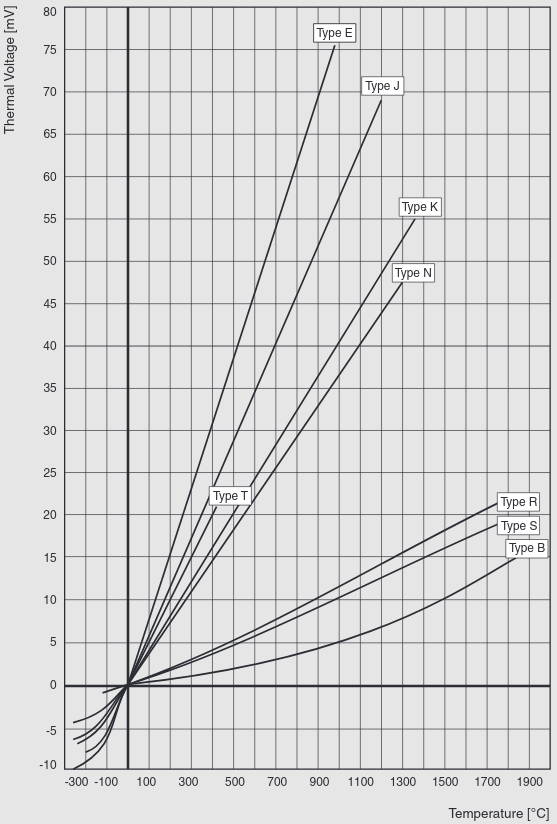
\includegraphics[width=0.6\linewidth]{./images/thermocouple-schema.png}
        \end{figure}

        \paragraph{}
        Ce graphique représente la caractéristique de transfert des différents types de thermocouple selon la norme EN 60584 à laquelle correspondent les deux thermocouples présentés. Par exemple, pour le thermocouple de type S, une tension de \SI{15}{\milli\volt} correspond à une température de \SI{1400}{\celsius}.


    \newpage
    \section{Effet pyroélectrique}

    \subsection{Définition}
    \paragraph{}
    Certains cristaux sont dits pyroélectriques lorsqu'ils présentent une polarisation électrique spontanée $P$ qui dépend de leur température $T$. Un changement de température dans ces cristaux entraîne une variation de leur polarisation qui peut engendrer un signal électrique qui, contrairement à l'effet thermoélectrique, est temporaire (il disparaît après le temps de relaxation diélectrique). La variation thermique de la polarisation est définie par le coefficient pyroélectrique $p$ : $$ p = \frac{\partial P}{\partial T}$$

    \paragraph{}
    L'effet pyroélectrique est utilisé dans les capteurs infrarouges, par exemple, pour détecter la présence d'un être humain ou animal à distance. Ils se basent sur le principe physique que tout corps émet des ondes infrarouges en relation avec la température du corps (Loi de Wien). Les rayons IR absorbés par le matériau pyroélec­trique élèvent sa température ce qui entraîne une modification de sa polarisation qui est mesurable par la variation de tension aux bornes d'un condensateur associé :
    \begin{figure}[H]
        \centering
        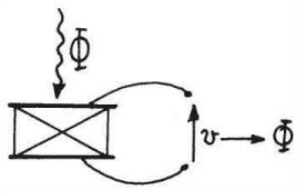
\includegraphics[width=0.2\linewidth]{./images/effet-pyro.png}
    \end{figure}

        \subsection{Capteurs infrarouges pyroélectriques (PIR)}
        \paragraph{}
    J'ai choisi deux capteurs infrarouges fabriqués par \href{https://www.murata.com/}{muRata} et \href{https://www.panasonic-electric-works.com/be/}{Panasonic}. Le mode de fonctionnement de ces capteurs dépend de l'effet pyroélectrique définit plus tôt : ils fournissent un signal électrique lorsqu'ils captent un changement de température (si la température devient ensuite stable, le signal cesse tout de même d'être produit). C'est capteurs sont conçus pour envoyer un signal lorsqu'une présence est détectée. Le signal de sortie étant un signal digital TOR, il s'agit donc plus à proprement parler de détecteurs que de capteurs. Les deux capteurs PIR sont vendus avec une lentille de Fresnel.
    
        \paragraph{}
        Les deux capteurs choisis peuvent être utilisés pour des applications variées : systèmes d'alarme (détection des intrusions), contrôle de lumière, de thermostats, etc.

        \subsubsection{Références}
        \begin{itemize}
            \item MuRata pyroelectric infrared sensor and lens IRA-S210ST01 IML-0688 : \url{https://www.murata.com/en-us/products/sensor/guide/sensorguide3/sensorguide/ira_imlseries}
            \item Panasonic AMN34112 - 10m Detection Type (long distance) : \url{https://www3.panasonic.biz/ac/e/search_num/index.jsp?c=detail&part_no=AMN34112&large_g_cd=1&medium_g_cd=14&small_g_cd=129&series_cd=1391}
        \end{itemize}

        \subsubsection{Comparaison de deux capteurs PIR}
            \begin{table}[H]
            \centering
            \begin{tabular}{l|c|c}
                \textbf{Modèle} & \textbf{MuRata IRA-S210ST01 IML-0688} & \textbf{Panasonic AMN34112}\\
                & 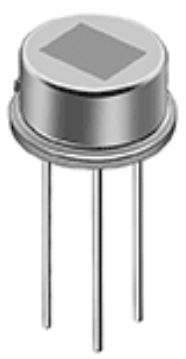
\includegraphics[width=0.1\linewidth]{./images/pyro-murata.png} & 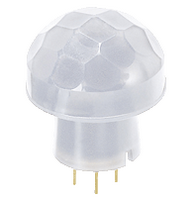
\includegraphics[width=0.2\linewidth]{./images/pyro-panasonic.png}\\
                \hline
                \textbf{Tension}            & de 2 à 15 VDC                                 & de -0.3 à 7 VDC\\
                \textbf{d'alimentation}     &                                               & \\
                \hline
                \textbf{Température}        & de -40 à 70\si{\celsius}                      & de -20 à 60\si{\celsius}\\
                \textbf{de fonctionnement}  & & \\
                \hline
                \textbf{Eléments}           & $2 \times (2.0 \times 1.0 \si{\milli\meter})$ & $4 \times (0.6 \times 0.6 \si{\milli\meter})$\\
                \textbf{pyroélectriques}    &                                               & \\
                \hline
                \textbf{Tension de sortie}  & min 3.6 mV                                    & entre 3 et 6 VDC \\
                \textbf{}                   & typiquement 4.6 mV                            & (car AOP intégré)\\
                \hline
                \textbf{Champ de détection} & & \\
                \textbf{-- Horizontal}      & \SI{35}{\degree} & \SI{93}{\degree}\\
                \textbf{-- Vertical}        & \SI{42}{\degree} & \SI{110}{\degree}\\
                \hline
                \textbf{Distance}           & --                                            & Longue distance :\\
                \textbf{de détection}       &                                               & $> 5 - 10 \si{\meter}$ \\
            \end{tabular}
            \end{table}

            \subsubsection{Schéma du circuit interne du capteur MuRata IRA-S210ST01}
            \begin{figure}[H]
                \centering
                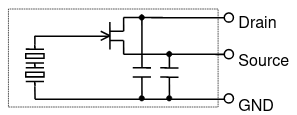
\includegraphics[width=0.4\linewidth]{./images/pyro-schema-circuit-diagram.png}
            \end{figure}

            \paragraph{}
            Ce schéma représente le circuit interne du capteur (de gauche à droite) : les deux éléments pyroélectriques et leur condensateur associé, un transistor JFET et deux condensateurs. Les trois sorties nous indiquent comment connecter le capteur : "Drain" pour la tension d'alimentation, "Source" pour la tension de sortie et "GND" pour la terre.

            \subsubsection{Schéma typique pour la détection d'un être humain}
            \begin{figure}[H]
                \centering
                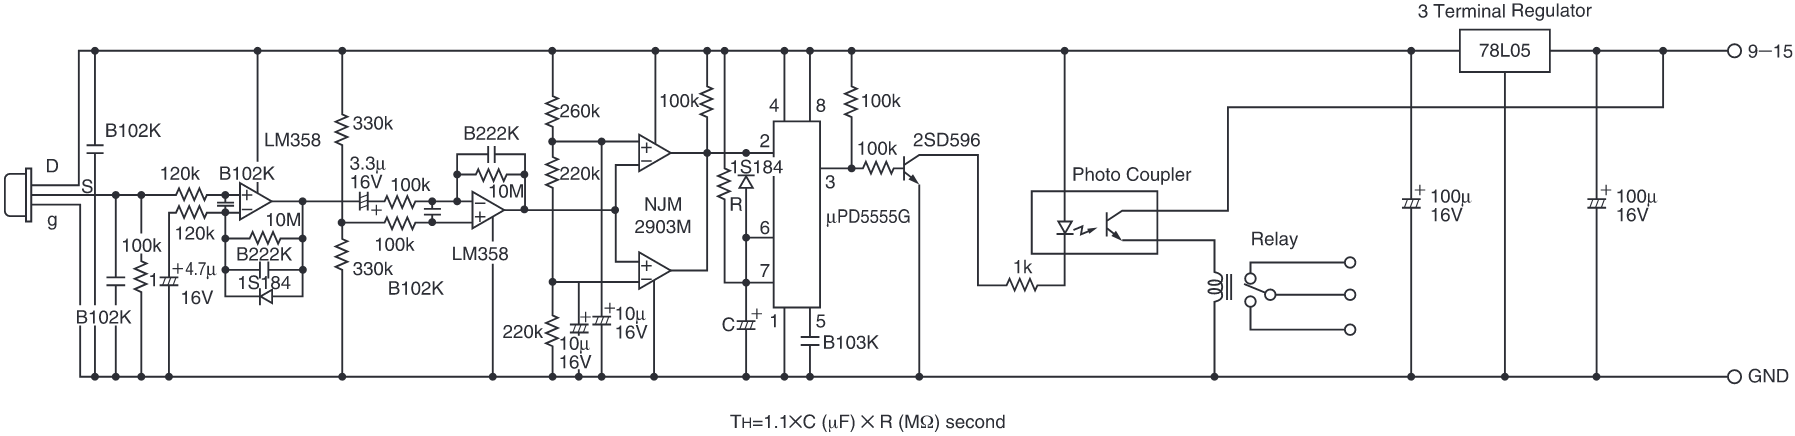
\includegraphics[width=\linewidth]{./images/pyro-schema-circuit-example.png}
            \end{figure}

            \paragraph{}
            Parmi les schémas fournis par le fabricant, celui-ci nous montre le circuit dans lequel intégrer le capteur PIR (à l'extrémité gauche) pour la détection d'un être humain.

    \newpage
    \section{Effet piézoélectrique}

    \subsection{Définition}
    \paragraph{}
    L'effet piézoélectrique permet de mesurer une force, une pression ou une accélération. Lorsqu'une contrainte mécanique est appliquée à certains matériaux dits piézoélectrique (e.g. le quartz), la déformation du matériau entraîne l'apparition de charges électriques égales et de signes contraires sur les faces opposées du matériau. En pratique, un condensateur est associé à l'élément piézoélectrique. Il est alors possible de mesurer une différence de potentiel aux bornes de ce condensateur proportinnelle à la force appliquée.

    \begin{figure}[H]
        \centering
        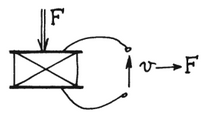
\includegraphics[width=0.2\linewidth]{./images/effet-piezo.png}
    \end{figure}

    \paragraph{}
    Dans le domaine des capteurs, l'effet piézoélectrique permet de mesurer une force et toutes les grandeurs s'y ramenant (pression, accélération, vibrations).

    \subsection{Capteurs de pression}
    \paragraph{}
    J'ai choisi deux capteurs de pression fabriqués par \href{https://sensing.honeywell.com/}{Honeywell} et par \href{https://www.anderson-negele.com/fr/}{Anderson-Negele}. Les deux capteurs fonctionnent sur la base d'une membrane en céramique présentant des propriétés piézoélectriques.

    \subsubsection{Références}
    \begin{itemize}
        \item Honeywell capteur de pression manométrique pour gaz secs modèle HSCDANN010BGAA5 : \url{https://sensing.honeywell.com/HSCDANN010BGAA5-amplified-board-mount-pressure-sensors}
        \item Anderson-Negele capteur de pression avec membrane céramique pour l'industrie alimentaire modèle DAC-341 : \url{https://www.anderson-negele.com/fr/p/capteurs-de-pression/dac-341/}
    \end{itemize}

    \subsubsection{Comparaison de deux capteurs de pression}
    \begin{table}[H]
        \centering
        \begin{tabular}{l|c|c}
            \textbf{Modèle} & \textbf{Honeywell HSCDANN010BGAA5} & \textbf{Anderson-Negele DAC-341}\\
                & 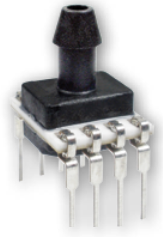
\includegraphics[width=0.15\linewidth]{./images/piezo-honeywell.png} & 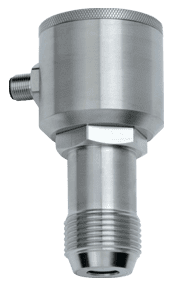
\includegraphics[width=0.15\linewidth]{./images/piezo-anderson-negele.png}\\
                \hline
                \textbf{Domaine}            & Médical (moniteurs de débit d'air,    & Industrie alimentaire (surveillance \\
                \textbf{d'application}      & machines d'anesthésie, d'analyse      & de la pression dans les brasseries, \\
                                            & de sang, etc.)                        & laiteries et industrie de boissons) \\
                                            & Industriel (barométrie, calibrateurs  & \\
                                            & de débit, chromographie de gaz, etc.) & \\
                \hline
                \textbf{Tension}            & 5 VDC                                 & 12 à 36 VDC                           \\
                \textbf{d'alimentation}     & & \\
                \hline
                \textbf{Type de pression}   & pression manométrique                 & pression absolue ou relative          \\
                \textbf{mesurée}            & & \\
                \hline
                \textbf{Plage de mesure}    & 0 à 10 bar                            & 0 à 20 bar                            \\
                \hline
                \textbf{Précision}          & $\pm 0,25 \%$                         & $\pm 0,25 \%$                         \\
                \hline
                \textbf{Signal de sortie}   & Analogique                            & Analogique                            \\
                                            & (boucle de courant de 4 à 20 mA)      & \\
            \end{tabular}
            \end{table}

            \subsubsection{Caractéristique de transfert du capteur de pression Honeywell}
            \begin{figure}[H]
                \centering
                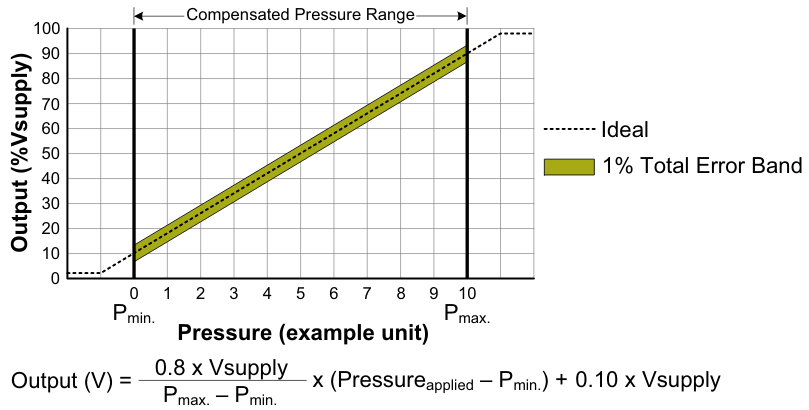
\includegraphics[width=0.7\linewidth]{./images/piezo-schema-caract-transfert.png}
            \end{figure}

            \paragraph{}
            Ce schéma nous donne la caractéristique de transfert du capteur ainsi que l'équation correspondant.

    
    \newpage
    \section{Effet photoélectrique}

    \subsection{Définition}
    \paragraph{}
    Les effets photoélectriques désignent la libération de charges électriques dans un matériau sous l'influence d'un rayonnement lumineux ou plus généralement électromagnétique, dont la longueur d'onde est inférieure à une valeur seuil, caractéristique du matériau. On distingue les effets photoélectriques internes et externes selon que les électrons arrachés sont émis hors du matériau ou pas. Lorsque les électrons sont libérés hors du matériau, il s'agit de l'effet photoémissif. Lorsqu'ils sont libérés à l'intérieur du matériau, il s'agit de l'effet photovoltaïque ou de la photoconductivité. 

    \paragraph{}
    Une cellule photoconductrice ou photorésistance permet de convertir une impulsion optique en impulsion électrique. Elle est constituée d'un matériau semiconducteur hautement résistif. Lorsqu'elle est soumise à un flux lumineux, des électrons sont libérées de la bande de valence pour atteindre la bande de conduction : sa résistance diminue alors et elle devient conductrice. 

    \begin{figure}[H]
        \centering
        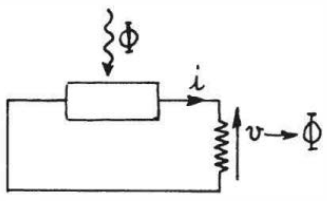
\includegraphics[width=0.3\linewidth]{./images/photoelec.png}
    \end{figure}

    \paragraph{}
    La cellule photoconductrice est typiquement utilisée pour commander un relais. Dans le domaine des capteurs, elle est utilisée pour la réception de signaux optiques dont la coupure peut permettre de de compter des objets, de mesurer la vitesse de rotation par disque tournant, etc.
    
    \paragraph{}
    La détection d'objets peut se faire de trois différentes façons :
    \begin{itemize}
        \item En barrage photoélectrique : les objets sont reconnus par l'interruption du faisceau entre un émetteur et un récepteur placés dans des boitiers séparés.
        \item En barrière reflex (capteurs autoréfléchissants) : les objets sont reconnus par l'interruption du faisceau émis, réfléchi (par un réflecteur) et réceptionné par un récepteur placé dans le même boitier que l'émetteur.
        \item En détecteur de réflexion directe (capteurs à diffusion) : les objets sont reconnus par la détection d'un faisceau réfléchi par ces objets et émis par un émetteur placé dans le même boitier que le récepteur. 
    \end{itemize}

    \subsection{Détecteurs reflex avec suppression d'arrière-plan}
    \paragraph{}
    J'ai choisi deux détecteurs d'objets fabriqués par \href{https://www.baumer.com/fr/fr/}{Baumer}. Ce sont deux détecteurs reflex avec élimination de l'arrière-plan (fonction qui permet de ne pas détecter les changements dans l'arrière plan à la place de l'objet que l'on souhaite détecter).

    \subsubsection{Références}
    \begin{itemize}
        \item Détecteur reflex modèle O500.GI-GW1B.72CU : \url{https://www.baumer.com/fr/fr/apercu-du-produits/detection-dobjets/barrieres-photoelectriques-et-detecteurs-reflex/standard-/o500-gi-gw1b-72cu/p/27392}
        \item Détecteur reflex modèle O300H.GL-GW1J.PVCV : \url{https://www.baumer.com/fr/fr/apercu-du-produits/detection-dobjets/barrieres-photoelectriques-et-detecteurs-reflex/miniatures/o300h-gl-gw1j-pvcv/p/27380}
    \end{itemize}

    \subsubsection{Comparaison de deux détecteurs reflex}
    \begin{table}[H]
        \centering
        \begin{tabular}{l|c|c}
        \textbf{Modèle}
            & \textbf{O500.GI-GW1B.72CU}
            & \textbf{O300H.GL-GW1J.PVCV}\\
            & 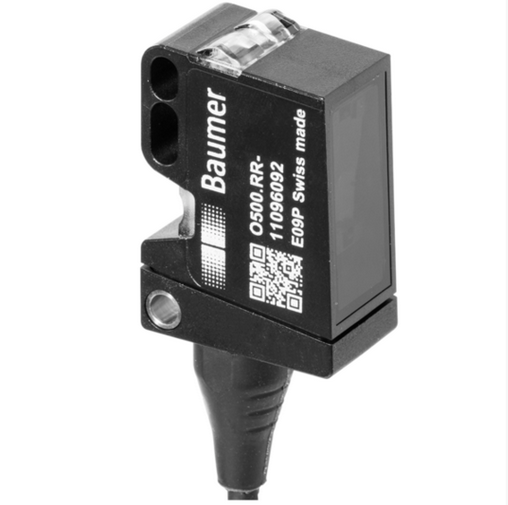
\includegraphics[width=0.2\linewidth]{./images/detect-reflex-A.png}
            & 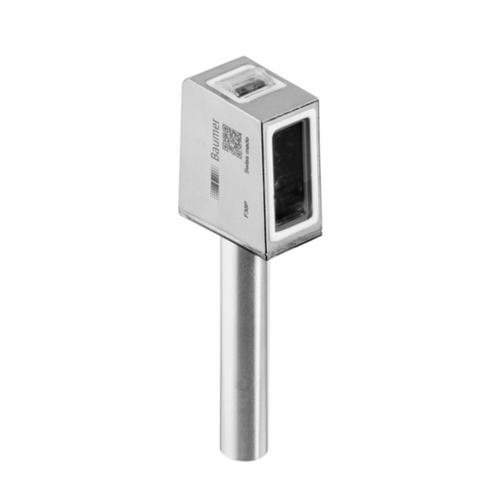
\includegraphics[width=0.2\linewidth]{./images/detect-reflex-B.png}\\
        \hline
        \textbf{Application}            & Détection avec élimination    & Détection avec élimination    \\
                                        & de l'arrière-plan             & de l'arrière-plan             \\
                                        &                               & Design hygiénique             \\
        \hline
        \textbf{Plage de détection}     & 30 à 600 mm                   & 30 à 250 mm                   \\
        \hline
        \textbf{Temps d'activation / }  & < 0,49 ms                     & < 0,25 ms                     \\
        \textbf{désactivation}          & & \\
        \hline
        \textbf{Protégé contre}         & & \\
        \textbf{-- les courts-circuits} & oui & oui \\
        \textbf{-- l'inversion de polarité} & oui & oui \\
        \hline
        \textbf{Circuit de sortie}      & push-pull                     & push-pull                     \\
        \hline
        \textbf{Classe de protection}   & IP67                          & IP 68/69K et proTect+         \\
    \end{tabular}
    \end{table}

    \subsubsection{Schéma de raccordement}

    \begin{figure}[H]
        \centering
        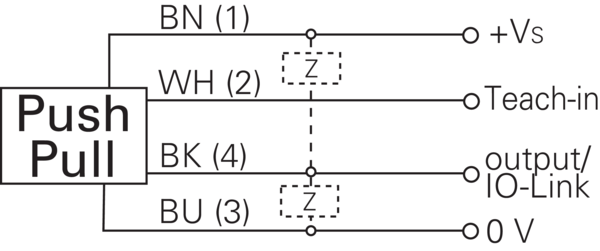
\includegraphics[width=0.3\linewidth]{./images/Zchn-5753-1.png}
    \end{figure}

    \paragraph{}
    Le détecteur a 4 câbles de raccordement : brun pour la tension d'entrée (entre 10 et 30V), blanc pour le réglage de la sensibilité, noir pour la sortie compatible avec IO-Link et bleu pour la terre.

    \paragraph{}
    Un push–pull est un circuit électronique cascode (composé de deux transistors de caractéristiques différentes) amplificateur de tension qui relie à la sortie deux composants actifs travaillant en opposition de phase, relié l'un au plus de l'alimentation, l'autre au moins. 


    \newpage
    \section{Effet photovoltaïque}

    \subsection{Définition}
    \paragraph{}
    L'effet photovoltaïque est un effet photoélectrique qui théorise la transformation d'énergie solaire (de lumière) en électricité. Il se présente généralement dans des matériaux semi-conducteurs hétérogènes (jonction PN ou PIN). Quand un photon interagit avec un électron de ce type de matériau, il cède sont énergie  à l'électron qui est alors libéré de sa bande de valence et migre vers la bande de conduction. Le trou correspondant migre en direction inverse. Le déplacement des paires électron-trou modifie la tension aux bornes de la cellule photovolaïque.
    
    \begin{figure}[H]
        \centering
        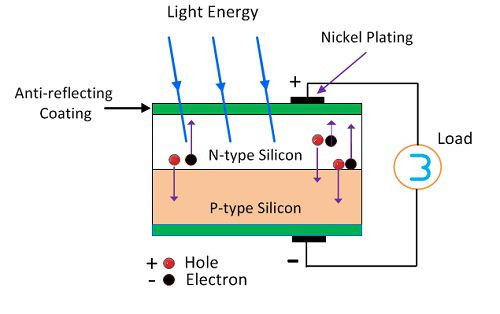
\includegraphics[width=0.5\linewidth]{./images/solar-cell.jpg}
    \end{figure}

    \paragraph{}
    La cellule photovoltaïque est le plus souvent utilisée comme générateur (panneaux photovoltaïques). Dans le domaine des capteurs, le composant le plus commun mettant en \oe uvre cet effet est la photodiode. La photodiode peut être utilisée à la fois en mode photoconducteur et en mode photovoltaïque. Utilisée en mode photovoltaïque, la photodiode se comporte comme un générateur : sous l'effet d'un flux lumineux, une tension proportionnelle à ce flux apparaît à ses bornes. On peut soit mesurer cette tension en circuit ouvert, soit le courant de court-circuit.

    \begin{figure}[H]
        \centering
        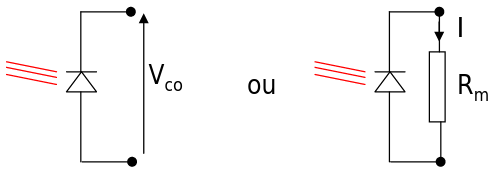
\includegraphics[width=0.4\linewidth]{./images/photodiode-photovltaique.png}
    \end{figure}

    \subsection{Choix de deux photodiodes}
    \paragraph{}
    J'ai choisi deux photodiodes fabriquées par \href{http://www.geni-uv.com/index.php}{GenUV}. Les deux photodiodes peuvent être utilisées en mode photovoltaïque. Elles permettent respectivement de détecter les UV A et les UV B.

    \subsubsection{Références}
    \begin{itemize}
        \item UV-A Sensor GUVA-S12SD : \url{http://www.geni-uv.com/download/products/GUVA-S12SD.pdf}
        \item UV-B Sensor GUVB-S11SD : \url{http://www.geni-uv.com/download/products/GUVB-S11SD.pdf}
    \end{itemize}

    \subsubsection{Comparaison de deux photodiodes}
    \begin{table}[H]
        \centering
        \begin{tabular}{l|c|c}
        \textbf{Modèle}
            & \textbf{UV-A Sensor GUVA-S12SD}
            & \textbf{UV-B Sensor GUVB-S11SD}\\
            & 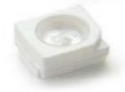
\includegraphics[width=0.1\linewidth]{./images/photodiode-UVA.png}
            & 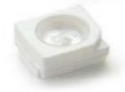
\includegraphics[width=0.1\linewidth]{./images/photodiode-UVA.png}\\
        \hline
        \textbf{Application}            & Détection des UV A            & Détection des UV B            \\
        \hline
        \textbf{Plage de détection}     & 240 à 370 \si{\nano\meter}    & 240 à 320 \si{\nano\meter}    \\
        \textbf{spectrale}              & & \\
        \hline
        \textbf{Plage de puissance}     & $0.1 \mu$ à \SI{100}{\milli\watt\per\square\centi\meter}& $0.1 \mu$ à \SI{100}{\milli\watt\per\square\centi\meter}\\
        \textbf{de la source optique}   & (Lampe UV A)                  & (Lampe UV B)                  \\
        \hline
        \textbf{Tension inverse max}    & 5 V                           & 3 V                           \\
        \hline
        \textbf{Courant direct max}     & \SI{1}{\milli\ampere}         & \SI{1}{\milli\ampere}         \\
        \hline
        \textbf{Température de}         & -30 à 85 \si{\celsius}        & -30 à 85 \si{\celsius}        \\
        \textbf{fonctionnement}         & & \\
    \end{tabular}
    \end{table}

    \subsubsection{Graphique de la courbe de responsivité de la photodiode pour UV B}

    \paragraph{}
    La figure (a) nous montre le fonctionnement de la photodiode. La responsivité est une grandeur physique mesurant le gain entrée/sortie d'un système de détection. Dans le cas spécifique des photodétecteurs, la responsivité mesure le courant électrique de sortie en fonction de la puissance optique d'entrée, et est un facteur de mérite du détecteur. La responsivité d'un photodétecteur est couramment exprimée en ampères par watt de puissance rayonnée incidente.

    \begin{figure}[H]
        \centering
        \begin{subfigure}[b]{0.418\linewidth}
            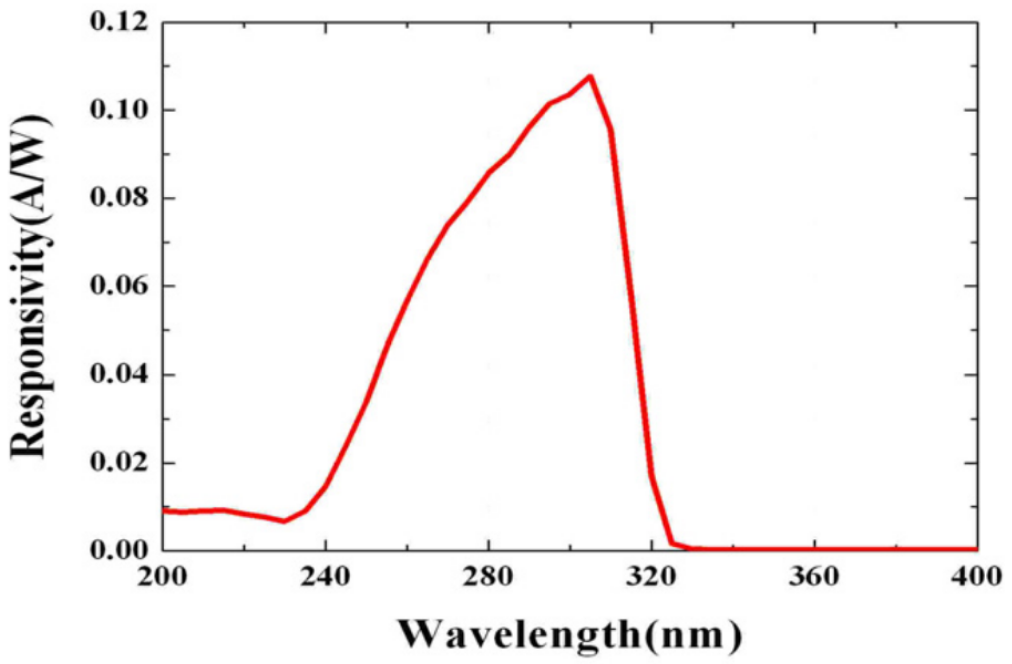
\includegraphics[width=\linewidth]{./images/photodiode-UVB-courbe-responsivite.png}
            \caption{Courbe de responsivité}
        \end{subfigure}
        \begin{subfigure}[b]{0.4\linewidth}
            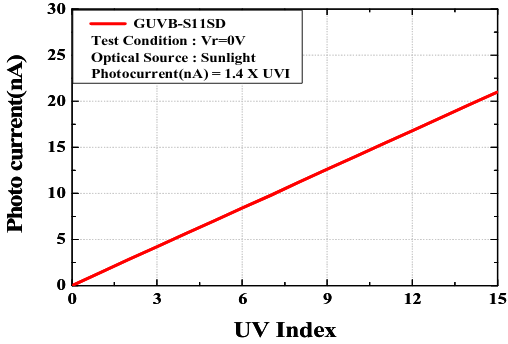
\includegraphics[width=\linewidth]{./images/photodiode-UVB-photocourant-indice-UV.png}
            \caption{Caractéristique de transfert}
        \end{subfigure}
    \end{figure}

    \paragraph{}
    Par exemple, pour une longueur d'onde de \SI{300}{\nano\meter}, le responsivité sera d'un peu plus de \SI{0.10}{\ampere\per\watt}.

    \subsubsection{Caractéristique de transfert}
    \paragraph{}
    La figure (b) nous permet d'interpréter les données de la photodiode. Elle représente la caractéristique de transfert de la photodiode : le photocourant émis par la photodiode en fonction de l'indice UV mesuré. L'indice UV est une échelle de mesure de l'intensité du rayonnement ultraviolet émis par le Soleil, et du risque qu'il représente pour la santé (plus l'indice est élevé, plus le risque pour la preau l'est aussi). Cette caractéristique est linéaire.
    

    \newpage
    \section{Effet photoémissif}

    \subsection{Définition}
    \paragraph{}
    L'effet photoémissif est un effet photoélectrique qui convertit un signal lumineux en signal électrique avec la particularité que les électrons arrachés du matériau par l'énergie lumineuse sont émis hors de ce matériau. Dans un capteur par photoémission, la photocathode est soumise au rayonnement et libère un nombre d'électrons proportionnel au nombre de photons incidents. Ces électrons émis par la photocathode forment le courant cathodique. Ils sont ensuite soit collectés directement par une anode (phototube à vide), soit à l'origine d'un processus multiplicatif qui entraîne une amplification du courant primaire : ionisation par chocs des molécules d'un gaz (phototube à gaz) ou émission secondaire (photomultiplicateur).

    \subsection{Photomultiplicateurs}
    \paragraph{}
    J'ai choisi deux photomultiplicaeurs fabriqués par \href{https://www.hamamatsu.com/}{Hamamatsu}, fabricant japonais spécialiste dans les appareils de mesure et d'émission de lumière et référence dans ce domaine. Les deux \href{https://www.hamamatsu.com/resources/pdf/etd/PMTmodules_TPMO0011E.pdf}{modèles choisis} sont des modules qui intègrent un photomultiplicateur à un circuit électronique.
    
    \paragraph{}
    En pratique, les tubes photomultiplicateurs sont capables de capter la lumière visible et au-delà du spectre visible pour l'\oe il humain et peuvent être utilisés comme compteurs de photons. Lorsque la lumière entre dans le tube, elle frappe la photocathode et des photoélectrons sont arrachés et émis dans l'enceinte sous vide du tube. Ces électrons sont attirés vers des électrodes secondaires (dynodes) portées à un potentiel supérieur. Le choc mécanique entre les électrons et chaque dynode crée des électrons secondaires qui sont émis sur chacune de ces dynodes. Le signal d'entrée est ainsi amplifié et apparait en sortie sur l'anode.

    \begin{figure}[H]
        \centering
        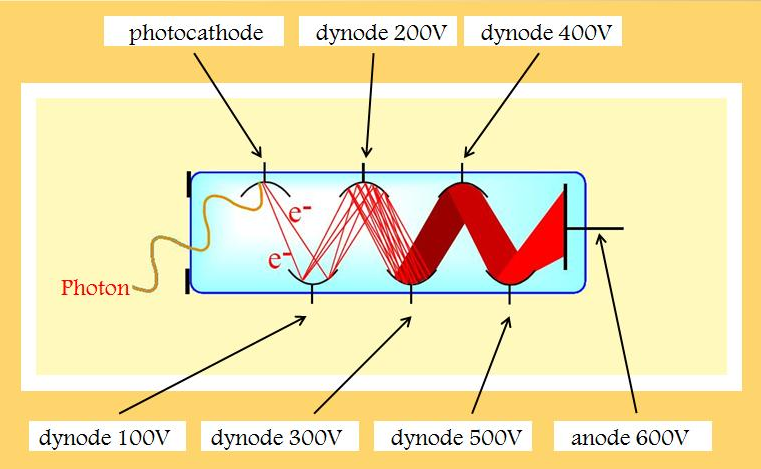
\includegraphics[width=0.6\linewidth]{./images/photomultiplicateur.png}
    \end{figure}

    \subsubsection{Références}
    \begin{itemize}
        \item Capteur de photons H9305-01 : \url{https://www.hamamatsu.com/eu/en/product/type/H9305-01/index.html}
        \item Compteur de photons H10682-110 : \url{https://www.hamamatsu.com/eu/en/product/type/H10682-110/index.html}
    \end{itemize}

    \subsubsection{Comparaison de deux modules à tube photomultiplicateur}
    \begin{table}[H]
        \centering
        \begin{tabular}{l|c|c}
        \textbf{Modèle}
            & \textbf{H9305-01}
            & \textbf{H10682-101}\\
            & 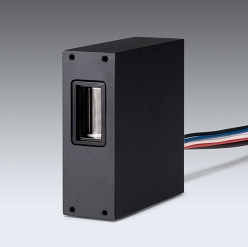
\includegraphics[width=0.2\linewidth]{./images/photomulti-H9305.png}
            & 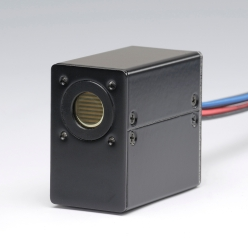
\includegraphics[width=0.2\linewidth]{./images/photomulti-H10682.png}\\
        \hline
        \textbf{Application}        & Cytométrie en flux        & Examen de sang        \\
        \textbf{typique}            & Puce de lecture ADN       & \\
                                    & Microscope multi-photons  & \\
        \hline
        \textbf{Longueur d'onde}    &  & \\
        \textbf{-- courte}          & \SI{185}{\nano\meter}     & \SI{230}{\nano\meter}     \\
        \textbf{-- longue}          & \SI{750}{\nano\meter}     & \SI{700}{\nano\meter}     \\
        \textbf{-- pic}             & \SI{420}{\nano\meter}     & \SI{400}{\nano\meter}     \\
        \hline
        \textbf{Tension d'entrée}   & 11.5 à 15 V               & 4.75 à 5.25 V\\
        \textbf{(max)}              & (18 V)                    & (6 V)\\
        \hline
        \textbf{Signal de sortie}   & Courant (max \SI{10}{\micro\ampere})  & Sortie logique\\
                                    &                                       & (logique positive)\\
        \hline
        \textbf{Temps de réponse}   & \SI{1.4}{\nano\second}    & --\\
        \hline
        \textbf{Température de}     & 5 à 50 \si{\celsius}      & 5 à 40 \si{\celsius}\\
        \textbf{fonctionnement}     & & \\
    \end{tabular}
    \end{table}

    \subsubsection{Schéma du module H10682-110}
    \begin{figure}[H]
        \centering
        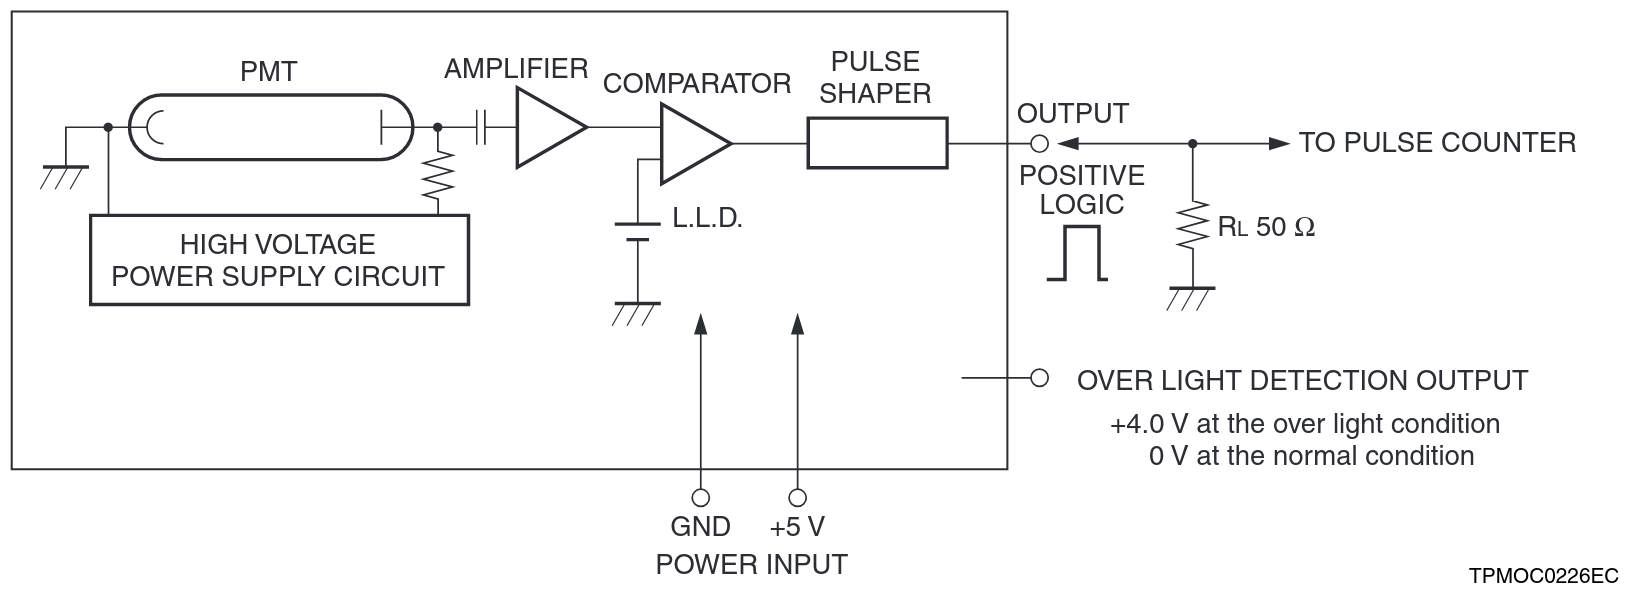
\includegraphics[width=0.8\linewidth]{./images/H10682-block-diagram.png}
    \end{figure}

    \paragraph{}
    Ce schéma représente le tube photomultiplicateur (PMT) et le circuit électronique qui lui est associé. Le module comprend un circuit d'alimentation. Le signal de sortie est amplifié puis comparé avant d'être mis en forme (impulsion de sortie pour la sortie logique). La résistance de la charge recommandée par ce schéma est de \SI{50}{\ohm}. Ce schéma montre également les entrées d'alimentation : alimentation en 5 V et terre.


    \newpage
    \section{Effet Hall}

    \subsection{Définition}
    \paragraph{}
    Lorsqu'un matériau (généralement semi-conducteur sous forme de plaquette) est parcouru par un courant $I$ et soumis à une induction $B$ faisant un angle $\theta$ avec le courant, une tension $v_H$ apparaît, dans une direction perpendiculaire à l'induction et au courant.
        
    \begin{figure}[H]
        \centering
        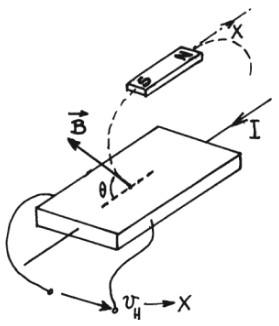
\includegraphics[width=0.3\linewidth]{./images/effet-hall.png}
    \end{figure}
            
    \paragraph{}
    Cette tension $v_H$ est fonction de $B$ et $\theta$, déterminés par la position de l'aimant. Elle a pour expression : $$v_H = K_H . I . \sin\theta$$ où $K_H$ dépend du matériau et des dimensions de la plaquette.
        
    \paragraph{}
    Dans le domaine des capteurs, l'effet Hall peut être utilisé pour déterminer la position d'un objet au moyen d'un aimant. Mais il est aussi utilisé pour détecter la présence d'un courant électrique ou d'un champ magnétique, pour mesurer un débit ou plus généralement toute grandeur basée sur la position (vitesse et accélération).
            
    \subsection{Codeurs incrémentaux pour servomoteurs et moteurs pas à pas}
    \paragraph{}
    J'ai choisi de comparer deux détecteurs de position incrémentaux pour servomoteurs ou moteurs pas à pas fabriqués par \href{https://www.posital.com/fr/}{Posital}. L'aimant est monté à l'extrémité de l'arbre du moteur et le codeur comporte 4 capteurs à effet Hall pour déterminer la position angulaire de l'axe du moteur \footnote{Voir \url{https://www.posital.com/fr/actualites/nouvelles-de-produit/standard_page_97.php}}.
            
    \subsubsection{Référence}
    \url{https://www.posital.com/fr/actualites/nouvelles-de-produit/stepper_kits.php}
        
    \subsubsection{Comparaison de deux codeurs incrémentaux}
    \begin{table}[H]
        \centering
        \begin{tabular}{l|c|c}
        \textbf{Modèle}
            & \textbf{KCD-BC01B-1617-E5XU-PRQ}
            & \textbf{KCD-BC01B-1617-E5XW-JAQ}\\
            & 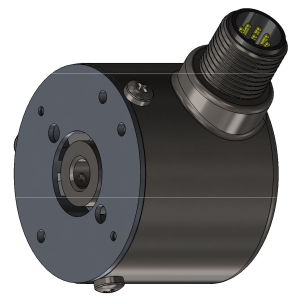
\includegraphics[width=0.2\linewidth]{./images/hall-KCD-BC01_B-1_617-E5XU-PRQ.png}
            & 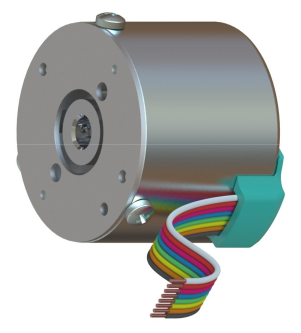
\includegraphics[width=0.2\linewidth]{./images/hall-KCD-S10_1B-1617-F7_XU-PRQ.png}\\
        \hline
        \textbf{Temps au démarrage}     & Max 1s                & Max 1s\\
        \hline
        \textbf{Résolution}             & 17 bits               & 17 bits\\
        \textbf{} & (16 bits en multitour) & (16 bits en multitour)\\
        \hline
        \textbf{Précision}              & $\le \pm$ 0,3 degré   & $\le \pm$ 0,3 degré\\
        \hline
        \textbf{Temps moyen de bon}     & 20 ans                & 20 ans\\
        \textbf{fonctionnement (MTTF)} & & \\
        \hline
        \textbf{Indice de protection}   & IP40                  & IP30 avec la fixation de câble\\
        \textbf{}                       &                       & IP20 sans la fixation de câble\\
        \hline
        \textbf{Connecteur électrique}  & M12, 8 pin            & JST SM08B-GHS-TB\\
    \end{tabular}
    \end{table}
        
    \subsubsection{Schéma de connexion du modèle KCD-BC01B-1617-E5XU-PRQ}
    \begin{figure}[H]
        \centering
        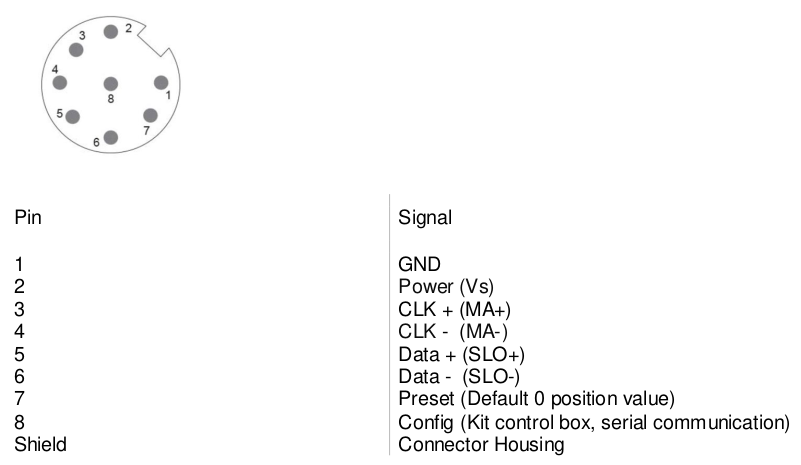
\includegraphics[width=0.7\linewidth]{./images/hall-schema.png}
    \end{figure}
    \paragraph{}
    Ce schéma montre quel signal est associé à chaque broche du connecteur M12 dont est pourvu le codeur incrémental KCD-BC01B-1617-E5XU-PRQ : la pin 1 doit être raccordée à la terre, la pin 2 à la tension d'alimentation (entre 4,75 et 15V continu), les pins 3 et 4 à l'horloge, les pins 5 et 6 aux données, la pin 7 permet de prérégler le capteur et la pin 8 permet de le configurer (i.e. de le calibrer).


    \newpage
    \addtocontents{toc}{\setcounter{tocdepth}{1}}
    \section*{Sources}

    \textbf{Général}
    \begin{itemize}
        \item Georges ASCH et coll., Les Capteurs en instrumentation industrielle, 7e édition, Dunod, Paris, 2010
        \item \url{https://perso.univ-st-etienne.fr/destoucn/Enseignements/CM-TD-CaptOpt.pdf}
        \item \url{http://cbissprof.free.fr/telechargements/tsiris/cours/capteurs.pdf}
        \item \url{http://www.sbaysite.net/sciences_ingenieur/Module3/Capteur/Les%20Capteurs.htm}
        \item \url{https://www.les-electroniciens.com/sites/default/files/cours/capteurs.pdf}
    \end{itemize}
    \bigskip

    \textbf{Effet thermoélectrique}
    \begin{itemize}
        \item \url{https://fr.wikipedia.org/wiki/Thermo%C3%A9lectricit%C3%A9}
        \item \url{https://fr.wikipedia.org/wiki/Effet_Seebeck}
        \item \url{https://fr.wikipedia.org/wiki/Thermocouple}
    \end{itemize}
    \bigskip

    \textbf{Effet pyroélectrique}
    \begin{itemize}
        \item \url{https://fr.wikipedia.org/wiki/Pyro%C3%A9lectricit%C3%A9}
        \item \url{https://fr.wikipedia.org/wiki/Lentille_de_Fresnel}
    \end{itemize}
    \bigskip

    \textbf{Photoélectricité}
    \begin{itemize}
        \item \url{https://fr.wikiversity.org/wiki/Capteur/Capteurs_optiques}
        \item \url{https://fr.wikipedia.org/wiki/Effet_photo%C3%A9lectrique}
        \item \url{https://fr.wikipedia.org/wiki/Photoconductivit%C3%A9}
        \item \url{https://fr.wikipedia.org/wiki/Responsivit%C3%A9}
        \item \url{https://fr.wikipedia.org/wiki/Cellule_photovolta%C3%AFque}
        \item \url{https://fr.wikipedia.org/wiki/Tube_photomultiplicateur}
    \end{itemize}

    % https://www.directindustry.fr/
\end{document}